\hyperdef{simple}{graphs}{\section{Simple Graphs}}

\subsection{Definition of Simple Graph}

Informally, a graph is a bunch of dots with lines connecting some of
them.  Here is an example:

\mfigure{!}{1.5in}{figures/graph-example.pdf}

For many Mathematical purposes, we don't really care how the points and
lines are laid out ---only which points are connected by lines.  The
definition of \emph{simple graphs} aims to capture just this connection
data.

\begin{definition}\label{graphdef} 
A \emph{simple graph}, $G$, consists of a nonempty set, $V$, called the
\emph{vertices} of $G$, and a collection, $E$, of two-element subsets of
$V$.  The members of $E$ are called the \emph{edges} of $G$.
\end{definition}

The vertices correspond to the dots in the picture, and the edges
correspond to the lines.  For example, the connection data in
dots-and-lines diagram above is a captured by the following simple graph:
\begin{eqnarray*}
V & = & \set{A, B, C, D, E, F, G, H, I} \\
E & = & \set{ \set{A, B}, \set{A, C}, \set{B, D}, \set{C, D},
              \set{C, E}, \set{E, F}, \set{E, G}, \set{H, I} }.
\end{eqnarray*}

It will be helpful to use the notation $\edge{A}{B}$ for the edge
$\set{A,B}$.  Note that $\edge{A}{B}$ and $\edge{B}{A}$ are different
descriptions of the same edge, since sets are unordered.

Two vertices in a simple graph are said to be \term{adjacent} if they are
joined by an edge, and an edge is said to be \term{incident} to the
vertices it joins.  The number of edges incident to a vertex is called the
\term{degree} of the vertex; equivalently, the degree of a vertex is
equals the number of vertices adjacent to it.  For example, in the simple
graph above, $A$ is adjacent to $B$ and $B$ is adjacent to $D$, and the
edge $\edge{A}{C}$ is incident to vertices $A$ and $C$.  Vertex $H$ has
degree 1, $D$ has degree 2, and $E$ has degree 3.

\subsubsection{Graph Synonyms}

A synonym for ``vertices'' is "nodes,'' and we'll use these words
interchangeably.

Simple graphs are sometimes called \emph{networks}, edges are sometimes
called \emph{arcs}, and adjacent vertices are sometimes called
\emph{neighbors}.  We mention this as a ``heads up'' in case you look at
other graph theory literature; we won't use these words.

Some technical consequences of Definition~\ref{graphdef} are worth noting
right from the start:
\begin{enumerate}
\item Simple graphs do not have edges going from a vertex
back around to itself (called a \emph{self-loop}).

\item There is at most one edge between two vertices of a simple graph.

\item Simple graphs have at least one vertex, though they might not have
any edges.
\end{enumerate}
There's no harm in relaxing these conditions, and some authors do, but we
don't need self-loops, multiple edges between the same two vertices, or
graphs with no vertices, and it's simpler not to have them around.

For the rest of these Notes we'll only be considering simple graphs, so
we'll just call them ``graphs'' from now on.

\hyperdef{sex}{america}{\subsection{Sex in America}\label{sexam}}

%A 1994 University of Chicago study entitled \textit{The Social
%Organization of Sexuality} found that on average men have 74\% more
%opposite-gender partners than women.

Let's model the question of heterosexual partners in graph theoretic
terms.  To do this, we'll let $G$ be the graph whose vertices, $V$, are
all the people in America.  Then we split $V$ into two separate subsets:
$M$, which contains all the males, and $F$, which contains all the
females.\footnote{For simplicity, we'll ignore the possibility of someone
  being both, or neither, a man and a woman.}  We'll put an edge between a
male and a female iff they have been sexual partners.  This graph is
pictured in Figure~\ref{fig:partners} with males on the left and females on
the right.

\begin{figure}[htbp]
\centering 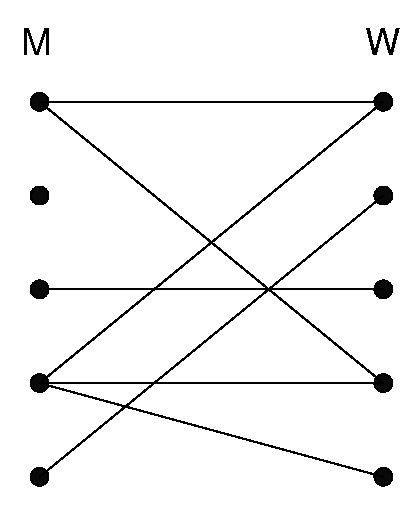
\includegraphics[height=1.75in]{figures/sex-edges.pdf}
\caption{The sex partners graph}
\label{fig:partners}
\end{figure}

Actually, this is a pretty hard graph to figure out, let alone draw.  The
graph is \emph{enormous}: the US population is about 300 million, so
$\card{V} \approx 300M$!  Of these, approximately 50.8\% are female and
49.2\% are male, so $\card{M} \approx 147.6M$, and $\card{F} \approx
152.4M$.  And we don't even have trustworthy estimates of how many edges
there are, let alone exactly which couples are adjacent.

But it turns out that we don't need to know any of this ---we just need to
figure out the relationship between the average number of partners per
male and partners per female.  To do this, we note that every edge is
incident to exactly one $M$ vertex (remember, we're only considering
male-female relationships); so the sum of the degrees of the $M$ vertices
equals the number of edges.  For the same reason, the sum of the degrees
of the $F$ vertices equals the number of edges.  So these sums are equal:
%
\[
\sum_{x \in M} \degr{x} = \sum_{y \in F} \degr{y}.
\]
%
Now suppose we divide both sides of this equation by the product of
the sizes of the two sets, $\card{M} \cdot \card{F}$:
%
\[
\left(\frac{\sum_{x \in M} \degr{x}}{\card{M}}\right) \cdot \frac{1}{\card{F}} =
\left(\frac{\sum_{y \in F} \degr{y}}{\card{F}}\right) \cdot \frac{1}{\card{M}}
\]
%
The terms above in parentheses are the \textit{average degree of an $M$
vertex} and the \textit{average degree of a $F$} vertex.  So we know:
\[
\text{Avg. deg in $M$} = \frac{\card{F}}{\card{M}} \cdot \text{Avg. deg in $F$}
\]

In other words, we've proved that the average number of female partners of
males in the population compared to the average number of males per
female is \emph{determined solely by the relative number of males and
females in the population}.

Now the Census Bureau reports that there are slightly more females than
males in America; in particular $\card{F} / \card{M}$ is about 1.035.  So
we know that on average, males have 3.5\% more opposite-gender partners
than females, and this tells us nothing about any sex's promiscuity or
selectivity.  Rather, it just has to do with the relative number of males
and females.  Collectively, males and females have the same number of
opposite gender partners, since it takes one of each set for every
partnership, but there are fewer males, so they have a higher ratio.  So the
University of Chicago, ABC, and the Federal government studies are way
off.  After a huge effort, they gave a totally wrong answer.

There's no definite explanation for why such surveys are consistently
wrong.  One hypothesis is that males exaggerate their number of partners
---or maybe females downplay theirs ---but these explanations are
speculative.  Interestingly, the principal author of the National Center
for Health Statistics study reported that she knew the results had to be
wrong, but that was the data collected and her job was to report that.

The same underlying issue has led to serious misinterpretations of other
survey data.  For example, a couple of years ago, the Boston Globe ran a
story on a survey of the study habits of students on Boston area campuses.
Their survey showed that on average, minority students tended to study
with non-minority students more than the other way around.  They went on
at great length to explain why this ``remarkable phenomenon'' might be
true.  But it's not remarkable at all ---using our graph theory
formulation, we can see that all it says is that there are fewer minority
students than non-minority students.  Well, that just follows from the
definition of ``minority''!

\subsection{Handshaking Lemma}

The previous argument hinged on the connection between a sum of degrees
and the number edges.  There is a simple connection between these in any
graph:

\begin{theorem}\label{sumedges}
The sum of the degrees of the vertices in a graph equals twice the number
of edges.
\end{theorem}

\begin{proof}
Every edge contributes two to the sum of the degrees, one for each of its
endpoints.
\end{proof}

Theorem~\ref{sumedges} is sometimes called the \emph{Handshake Theorem}:
if we total up the number of people each person at a party shakes hands
with, the total will be twice the number of handshakes that occurred.

\subsection{Some Common Graphs}

Some graphs come up so frequently that they have names.  The {\em complete
graph} on $n$ vertices, also called $K_n$, has an edge between every two
vertices.  Here is $K_5$:

\mfigure{!}{1.5in}{figures/complete-graph.pdf}

The {\em empty graph} has no edges at all.  Here is the
empty graph on 5 vertices:

\mfigure{!}{1.5in}{figures/empty-graph.pdf}

Another 5 vertex graph is $L_4$, the \emph{line graph} of length four:

\mfigure{!}{1in}{figures/path-graph.pdf}

And here is $C_5$, a \emph{simple cycle} with 5 vertices:

\mfigure{!}{1.5in}{figures/cycle.pdf}

\subsection{Isomorphism}

Two graphs that look the same might actually be different in a formal
sense.  For example, the two graphs below are both simple cycles with
4~vertices:

\mfigure{!}{1.5in}{figures/isomorphism.pdf}

But one graph has vertex set $\set{A, B, C, D}$ while the
other has vertex set $\set{1, 2, 3, 4}$.  If so, then the graphs are
different mathematical objects, strictly speaking.  But this is a
frustrating distinction; the graphs {\em look the same}!

Fortunately, we can neatly capture the idea of ``looks the same.''  Graphs
$G_1$ and $G_2$ are {\em isomorphic} if there exists a bijection between
the vertices in $G_1$ and the vertices in $G_2$ such that there is an edge
between two vertices in $G_1$ if and only if there is an edge between the
two corresponding vertices in $G_2$.  For example, take the following
bijection between vertices in the two graphs above:
\[
\begin{array}{lll}
A \text{ corresponds to } 1 & \hspace{0.5in} & B \text{ corresponds to } 2 \\
D \text{ corresponds to } 4 & & C \text{ corresponds to } 3.
\end{array}
\]
Now there is an edge between two vertices in the graph on the left if and
only if there is an edge between the two corresponding vertices in the
graph on the right.  Therefore, the two graphs are isomorphic.  The
bijection itself is called an {\em isomorphism}.
\begin{definition}
If $G_1$ is a graph with vertices, $V_1$, and edges,
$E_1$, and likewise for $G_2$, then $G_1$ is {\em isomorphic} to $G_2$ iff
there exists a \textbf{bijection}, $f: V_1 \to V_2$, such that for
every pair of vertices $u, v \in V_1$:
\[
\edge{u}{v} \in E_1 \qiff \edge{f(u)}{f(v)} \in E_2.
\]
The function $f$ is called an {\em isomorphism} between $G_1$ and
$G_2$.
\end{definition}

Two isomorphic graphs may be drawn very differently.  For example, here
are two different ways of drawing $C_5$:

\mfigure{!}{1.5in}{figures/isomorphism-c5.pdf}

Isomorphism captures all the connection properties of a graph, abstracting
out what the vertices are called, what they are made out of, or where they
appear in a drawing of the graph.  So a property like ``having three
vertices of degree 4'' is preserved under isomorphism, while ``having a
vertex that is an integer'' is not preserved.  In particular, if one graph
has three vertices of degree 4 and another does not, they can't be
isomorphic.  Similarly, if one graph has an edge that is incident to
a degree 8 vertex and a degree 3 vertex, then any isomorphic graph must also
have such an edge.

Looking for properties like these can make it easy to determine that two
graphs are not isomorphic, or to actually find an isomorphism between
them, if there is one.  In practice, it's frequently easy to decide
whether two graphs are isomorphic.  However, no one has yet found a
\emph{general} procedure for determining whether two graphs are isomorphic
which is \emph{guaranteed} to run much faster than an exhaustive (and
exhausting) search through all possible bijections between their
vertices.

Having an efficient procedure to detect isomorphic graphs would, for
example, make it easy to search for a particular molecule in a database
given the molecular bonds.  On the other hand, knowing there is no such
efficient procedure would also be valuable: secure protocols for
encryption and remote authentication can be built on the hypothesis that
graph isomorphism is computationally exhausting.

\endinput